\documentclass[a4paper]{article}

\usepackage[utf8]{inputenc}
\usepackage[DIV=12]{typearea}
\usepackage{microtype}
\usepackage{mathtools, amssymb, bm}
\usepackage{parskip}
\usepackage{subcaption}
\usepackage{float}
\usepackage[shortlabels]{enumitem}
\usepackage[colorlinks=true]{hyperref}
\hypersetup{linktoc=all}

\title{3}
\date{} 

\begin{document}
\maketitle
We generated results for two kinds of random matrices, one with entries from the standard normal distribution (\texttt{randn}) and the other from standard uniform distribution (\texttt{rand}). And then, their $r$ rank approximation was taken. The plots are given below, the exact RMSE values are saved in the media directory.
\begin{figure}[H]
	\centering
	\begin{subfigure}{0.45\linewidth}
		\centering
		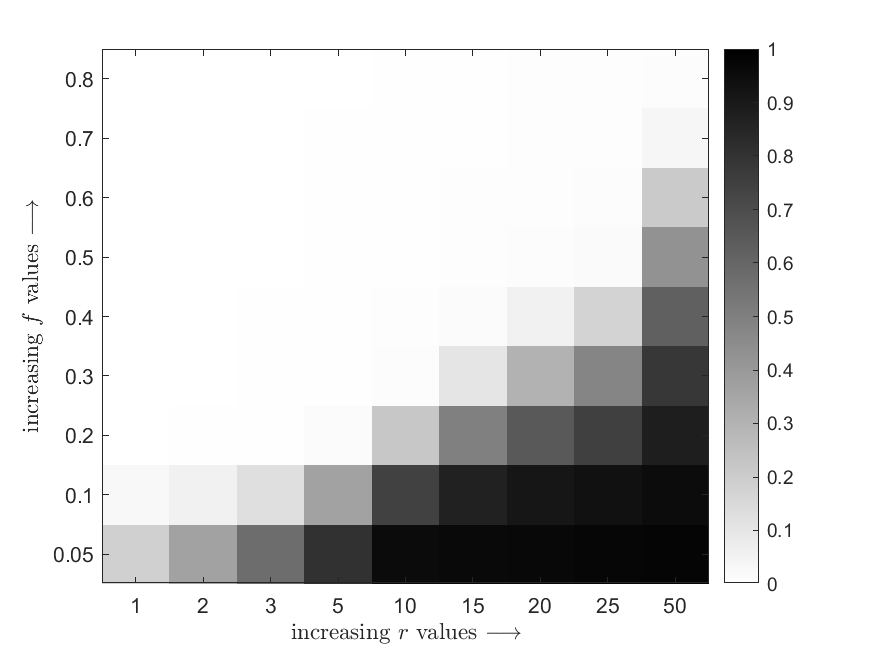
\includegraphics[width=\linewidth]{../media/Q2 randn RMSEs.png}
		\caption{\texttt{randn}}
	\end{subfigure}
	\begin{subfigure}{0.45\linewidth}
		\centering
		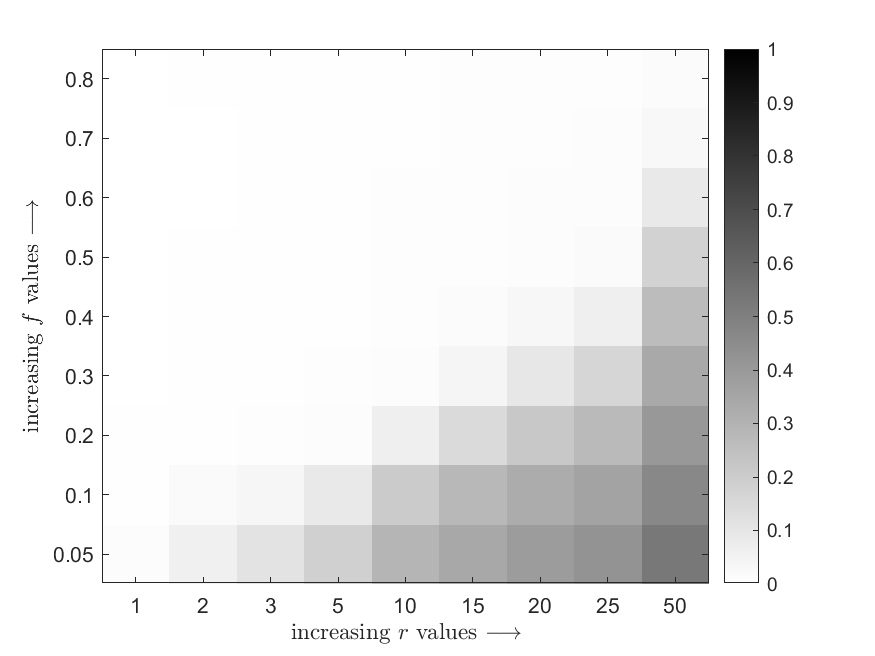
\includegraphics[width=\linewidth]{../media/Q2 rand RMSEs.png}
		\caption{\texttt{rand}}
	\end{subfigure}
	\caption{Both figures with the same color scale for better comparison}
\end{figure}
\section{Observations}
\begin{itemize}
\item RMSE values of random matrices generated using values from guassian distribution are significantly greator compared to the random matrices with uniform distribution. A possible reason could be as there is a clear dominant eigenvalue (magnitude) in the latter case while no such eigenvalue in the former case.
\item As rank increases, RMSE increases implying worsening reconstruction.
\item As number of measurements increases, RMSE decreases implying improving reconstruction.
\end{itemize}
\end{document}